\section{Onderzoeksonderwerpen}
Voor het onderzoeksrapport moeten alle opties worden uitgezocht voor de mogelijke manieren van implementatie van het project. Om	 te beginnen moet er worden bestudeerd hoe het huidige systeem precies werkt. Zo moet er worden uitgezocht welke frameworks er als beste kunnen worden gebruikt. Enerzijds een framework voor het datatransport, anderzijds een framework voor de GUI. Daarnaast moet ook worden gekeken op welke manier de data van het exoskelet naar de externe bron moet worden verzonden. Hiervoor moet zowel naar hardware als software worden gekeken.
\subsection{Hoe werkt het huidige systeem}
In het huidige systeem wordt met behulp van Simulink alle gegevens uit de sensoren bijeengeraapd. Hoe dit precies werkt moet nog worden uitgezocht. 
\subsection{Model}
Voor het model is het huidige idee om de data van het exoskelet naar een receiver te sturen. De schoont dan de data op, en stuurt deze door naar mogelijk meerdere instanties van de interface.
\begin{figure}[!ht]
	\centering
	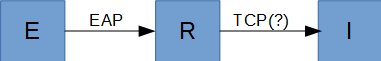
\includegraphics[width=150px]{ERIModel}
	\caption{Schematische weergave van het model. \textit{E} staat voor het exoskelet, \textit{R} staat voor de receiver en \textit{I} staat voor de interface.}
\end{figure}
\subsection{Frameworks}
\subsubsection{GUI}
Voor de GUI is een framework nodig wat 3D-visualisatie ondersteunt.
\subsubsection{Dataverbinding naar GUI}
Er is een Framework nodig dat de data die binnenkomt in Simulink omzet in data die kan worden gebruikt door de GUI. Hierbij moet rekening worden gehouden met het feit dat MatLab een beperkt aantal talen ondersteunt.
\subsection{Connectiviteitsopties}
\subsubsection{Hardware}
Er is momenteel nog geen hardware beschikbaar om de data draadloos te zenden van het exoskelet naar de receiver. Het exoskelet heeft zowel een USB-poort als een Ethernet-poort, wat de opties voor mogelijke hardware redelijk uitgebreid maakt.
\subsubsection{Software}
Het beoogde protocol om de data te verzenden is momenteel EtherCat. EtherCat lijkt alle functionaliteiten te hebben die worden verwacht nodig te zijn. 